%%%%%%%%%%%%%%%%%%%%%%%%%%%%%%%%%%%%%%%%%%%%%%%%%%%%%%%%%%%%%%%%%%%%%%%%%%%%%%%
%% StuPro B, "Programmierumgebung Offener Antrieb" (POA)
%% Angebot
%% $Id: handbuch.tex,v 1.3 2004/02/06 00:25:16 neco Exp $
%%%%%%%%%%%%%%%%%%%%%%%%%%%%%%%%%%%%%%%%%%%%%%%%%%%%%%%%%%%%%%%%%%%%%%%%%%%%%%%
\documentclass[a4paper,titlepage,12pt,ngerman]{scrbook}
\usepackage{.../common/header}

\RCSdef $Revision: 1.3 $
\RCSdef $Date: 2004/02/06 00:25:16 $

\newcommand\version{Version 1.0 \xspace}

\begin{document}

%%%%%%%%%%%%%%%%%%%%%%%%%%%%%%%%%%%%%%%%%%%%%%%%%%%%%%%%%%%%%%%%%%%%%%%%%%%%%%%
%% Deckblatt

\begin{titlepage}
\renewcommand{\thefootnote}{\fnsymbol{footnote}}
{\Huge
\raggedright
\textbf{POA} \\
\huge Programmierumgebung offener Antrieb
\rule{\textwidth}{0.75pt}
\par
}
\begin{flushleft}
\normalsize
\version
\end{flushleft}
\vfill

{\parindent=0cm
\Huge Handbuch
}


\setcounter{footnote}{0}
\end{titlepage}


%%%%%%%%%%%%%%%%%%%%%%%%%%%%%%%%%%%%%%%%%%%%%%%%%%%%%%%%%%%%%%%%%%%%%%%%%%%%%%%
%% Inhaltsverzeichnis

\tableofcontents

%%%%%%%%%%%%%%%%%%%%%%%%%%%%%%%%%%%%%%%%%%%%%%%%%%%%%%%%%%%%%%%%%%%%%%%%%%%%%%%
%%%%%%%%%%%%%%%%%%%%%%%%%%%%%%%%%%%%%%%%%%%%%%%%%%%%%%%%%%%%%%%%%%%%%%%%%%%%%
%%%%%%%%%%%%%%%%%%%%%%%%%%%%%%%%%%%%%%%%%%%%%%%%%%%%%%%%%%%%%%%%%%%%%%%%%%%%%
\chapter{Einleitung}
\section{Die Motivation f"ur POA}

Es werden viele Neuentwicklungen im Bereich der Werkzeugmaschinen gemacht.
Viele dieser Entwicklungen beinhalten neue Kinematiken, wie z.B. die
Parallelkinematiken und Sensoren (z.B. den Ferraris 
Relativbeschleunigungssensor).
Dadurch entstehen neue Anforderungen an die Antriebsregelung. Zus"atzliche
Sensor-Signale m"ussen in den Reglerstrukturen ber"ucksichtigt werden -- oder
es werden sogar v"ollig neue Reglerstrukturen ben"otigt.\par
Die momentan auf dem Markt erh"altlichen Reglersysteme erlauben meist
weder die Ber"ucksichtigung neuartiger Sensoren, noch bieten sie die
M"oglichkeit, eigene anwenderspezifische Reglerstrukturen zu implementieren.\par
Daher wird am ISW eine Plattform f"ur die Antriebsregelung entwickelt,
auf der es dem Anwender in jeder Hinsicht offen steht, eigene Funktionalit"aten
zu integrieren. Diese Plattform wird am ISW kurz als ``Offener Antrieb''
bezeichnet.  \par
Die hardwaretechnische Realisierung erfolgt in Form einer PC-Einsteckplatine.
Zentrales Element des Offenen Antriebes ist der Altera ``APEX'' Baustein. Es
handelt sich dabei um ein CPLD\footnote{Complex Programmable Logic Device},
das sich frei programmieren l"asst. Der Anwender hat die M"oglichkeit, die
Funktion des Bausteins seinen Bed"urfnissen anzupassen.\par
Um die Offenheit f"ur jeden Anwender nutzbar zu machen, wird f"ur das CPLD eine
Architektur festgelegt, die es erm"oglicht, einzelne Funktionalit"aten in Form
von Modulen zu implementieren. Diese Module k"onnen aus festprogrammierten
Schaltungen (Cores) und freiprogrammierbaren CPUs bestehen. Jedes Modul kann
auf die Signale aller anderen Module zugreifen und stellt seine eigenen
Ausgangssignale allen anderen Modulen zur Verf"ugung.\par
POA bietet eine anwenderfreundliche Programmierumgebung f"ur das Netzwerk
von CPUs und Cores, in dem ein bereits auf dem CPLD vorhandenes
Netzwerk konfiguriert werden kann.



%%%%%%%%%%%%%%%%%%%%%%%%%%%%%%%%%%%%%%%%%%%%%%%%%%%%%%%%%%%%%%%%%%%%%%%%%%%%%

\chapter{Funktionalit"at von POA}

 POA bietet im wesentlichen diese Funktionalit"aten:
\begin{itemize}
\item Darstellung und Manipulation rasterisierter CPLD Layouts
\item Verwaltung und Editierung einer CPLD-Modulbibliothek zur CPLD-Layout
      Manipulation
\item Rahmencodegenerierung f"ur eingebette CPU-Module in einem CPLD-Layout
\item Plausibilit"atspr"ufung und Optimierung eines entworfenen CPLD-Layouts
\item Compilieren und Herunterladen von Quellcode f"ur die CPU-Module
\item Speichern und "Offnen von CPLD-Layouts und zugeh"origem Quellcode
\item Konfiguration der Programmeigenschaften
\item Zusammenarbeit mit externen Programmen
\end{itemize}
Auf die Einzelheiten der wesentlichen Funktionalit"aten wird in den folgenden Abschnitten eingegangen.


%%%%%%%%%%%%%%%%%%%%%%%%%%%%%%%%%%%%%%%%%%%%%%%%%%%%%%%%%%%%%%%%%%%%%%%%%%%%%

\chapter{Installation von POA}

\section{Systemanforderungen an POA}
POA ist f"ur verschiedene Betriebssysteme verf"ugbar:
\begin{itemize}
\item 32-Bit-Windows (95/98/ME/NT4.0/2000/XP)
\item Linux
\end{itemize}


\subsection{Installation unter Linux}
	
\subsection{Installation unter Windows}


%%%%%%%%%%%%%%%%%%%%%%%%%%%%%%%%%%%%%%%%%%%%%%%%%%%%%%%%%%%%%%%%%%%%%%%%%%%%%
	
\chapter{Die graphische Bedieneroberfl"ache}

\section{Das Hauptfenster}
\begin{figure}[htbp]

\begin{center}

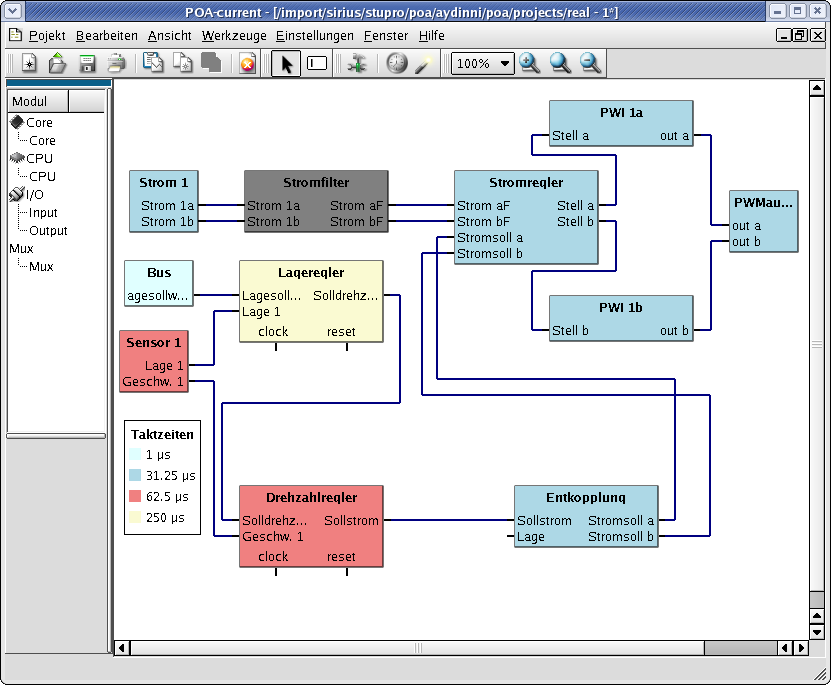
\includegraphics[width=10cm]{Mainwindow1}

\caption{Mainwindow}\label{test}

\end{center}

\end{figure}

Die Menueleiste besteht aus den Menues Project, Edit, View, Tools, Settings, Windows und Help.

\begin{itemize}
\item Project:	New, Open, Save, Save as, Print, Recent, Exit.
\item Edit: 	Cut, Copy, Paste
\item View: 	Zoom in, Zoom normal, Zoom out 
\item Tools: 	Configuration, Route, Scheduling, Deploy Project
\item Settings:	Show Grid, Configure POA
\item Windows: 	Tile, Tile Horizotal, Cascade
\item Help: 	Contens, About
\end{itemize}

Die meisten Aktionen k"onnen auch schneller mit den Befehlsbuttons in der Symbolleiste ausgef"uhrt werden.
	
\section{Dialogboxen}

\subsection{CPU Konfiguration Dialogbox}
\subsection{I/O Block Konfiguration Dialogbox}
\subsection{Scheduling Dialogbox}
\subsection{Datei Dialogbox}

%%%%%%%%%%%%%%%%%%%%%%%%%%%%%%%%%%%%%%%%%%%%%%%%%%%%%%%%%%%%%%%%%%%%%%%%%%%%%
%%%%%%%%%%%%%%%%%%%%%%%%%%%%%%%%%%%%%%%%%%%%%%%%%%%%%%%%%%%%%%%%%%%%%%%%%%%%%

\chapter{Anleitung}


%%%%%%%%%%%%%%%%%%%%%%%%%%%%%%%%%%%%%%%%%%%%%%%%%%%%%%%%%%%%%%%%%%%%%%%%%%%%%
\section{POA konfigurieren}

\subsection{Raster einstellen}
\begin{figure}[htbp]

\begin{center}

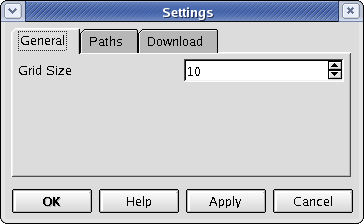
\includegraphics[width=10cm]{POAConfiguration1}

\caption{POA Configuration}\label{test}

\end{center}

\end{figure}
W"ahlen Sie im Untermenue von {\bf Settings} den Eintrag {\bf Configure POA..}. Im aufklappenden Dialog k"onnen Sie unter dem Dateireiter {\bf General} die gew"unschte Raster Gr"o"se eingeben.\par
Mit {\bf OK} werden die Einstellungen f"ur das Projekt gespeichert.\par
Mit {\bf Apply} werden die Einstellungen "ubernommen.\par
Mit {\bf Cancel} werden die Einstellungen verworfen.\par 

\subsection{Externe Programme einbinden}
\begin{figure}[htbp]

\begin{center}

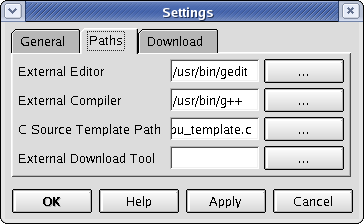
\includegraphics[width=10cm]{POAConfiguration2}

\caption{POA Configuration}\label{test}

\end{center}

\end{figure}
W"ahlen Sie im Untermenue von {\bf Settings} den Eintrag {\bf Configure POA..}. Im aufklappenden Dialog k"onnen Sie unter dem Dateireiter {\bf Paths} die gew"unschten externen Programme einbinden.
\subsubsection{Externen Editor einbinden}
Um einen Editor einzubinden, w"ahlen Sie unter dem Dateireiter {\bf Paths} das Textfeld neben {\bf External Editor} aus und geben Sie hier den korrekten Pfad des Editors ein. Alternativ dazu k"onnen Sie auch mit dem Button neben dem Textfeld im Verzeichnisbaum nach dem gew"unschten Editor suchen.\par
Mit {\bf OK} werden die Einstellungen f"ur das Projekt gespeichert.\par
Mit {\bf Apply} werden die Einstellungen "ubernommen.\par
Mit {\bf Cancel} werden die Einstellungen verworfen.\par 

\subsubsection{Externen Compiler einbinden}
Um einen Compiler einzubinden, w"ahlen Sie unter dem Dateireiter {\bf Paths} das Textfeld neben {\bf External Compiler} aus und geben Sie hier den korrekten Pfad des Compilers ein. Alternativ dazu k"onnen Sie auch mit dem Button neben dem Textfeld im Verzeichnisbaum nach dem gew"unschten Compiler suchen.\par
Mit {\bf OK} werden die Einstellungen f"ur das Projekt gespeichert.\par
Mit {\bf Apply} werden die Einstellungen "ubernommen.\par
Mit {\bf Cancel} werden die Einstellungen verworfen.\par 

\subsubsection{Externen Download Tool einbinden}
Um einen Download Tool einzubinden, w"ahlen Sie unter dem Dateireiter {\bf Paths} das Textfeld neben {\bf External Download Tool} aus und geben Sie hier den korrekten Pfad des Download Tool ein. Alternativ dazu k"onnen Sie auch mit dem Button neben dem Textfeld im Verzeichnisbaum nach dem gew"unschten Download Tool suchen. \par
Mit {\bf OK} werden die Einstellungen f"ur das Projekt gespeichert.\par
Mit {\bf Apply} werden die Einstellungen "ubernommen.\par
Mit {\bf Cancel} werden die Einstellungen verworfen.\par 

\subsection{C Source Template Pfad angeben}
Um einen C Source Template Pfad anzugeben, w"ahlen Sie unter dem Dateireiter {\bf Paths} das Textfeld neben {\bf C Source Template Path} aus und geben Sie hier den korrekten Pfad ein. Alternativ dazu k"onnen Sie auch mit dem Button neben dem Textfeld im Verzeichnisbaum nach dem gew"unschten Pfad suchen. \par
Mit {\bf OK} werden die Einstellungen f"ur das Projekt gespeichert.\par
Mit {\bf Apply} werden die Einstellungen "ubernommen.\par
Mit {\bf Cancel} werden die Einstellungen verworfen.\par 

\subsection{Download Einstellung}
\begin{figure}[htbp]

\begin{center}

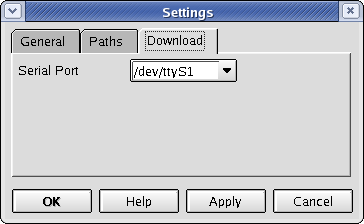
\includegraphics[width=10cm]{POAConfiguration3}

\caption{POA Configuration}\label{test}

\end{center}

\end{figure}
F"ur Downloadeinstellungen w"ahlen Sie den Datiereiter {\bf Download}. Hier k"onnen Sie in der Kombobox den Seriellen Port einstellen.\par 
Mit {\bf OK} werden die Einstellungen f"ur das Projekt gespeichert.\par
Mit {\bf Apply} werden die Einstellungen "ubernommen.\par
Mit {\bf Cancel} werden die Einstellungen verworfen.\par 


%%%%%%%%%%%%%%%%%%%%%%%%%%%%%%%%%%%%%%%%%%%%%%%%%%%%%%%%%%%%%%%%%%%%%%%%%%%%%
\section{Ein Projekt anlegen, "offnen, speichern}
\begin{figure}[htbp]

\begin{center}

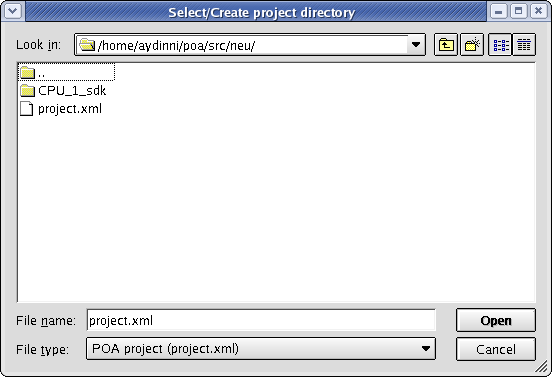
\includegraphics[width=10cm]{Directory}

\caption{Projekt Directory}\label{test}

\end{center}

\end{figure}

\subsection{Neues Projekt anlegen}
Druch anklicken des Menues {\bf Project} in der Menueleiste erscheint ein Untermenue {\bf New}. Wenn Sie dies ausw"ahlen, wird eine Dialogbox ge"offnet, in der Sie den Pfad f"ur das neue Projekt anlegen k"onnen.\par
Mit {\bf OK} werden die Einstellungen "ubernommen.\par
Mit {\bf Cancel} werden die Einstellungen verworfen.\par
Ein neues Projekt kann auch durch Mouseklick auf das Symbol {\bf New} in der Symbolleiste angelegt werden.
Wird ein neues Projekt angelegt, dann wird dadurch auch das Arbeitsfenster im Hauptfenster aktiviert.

\subsection{Bestehendes Projekt "offnen}
Im Untermenue von {\bf Project} den Eintrag {\bf Open} oder in der Symbolleiste den {\bf Ordner} anklicken. Im nun aufklappendem Dialog k"onnen Sie im Verzeichnisbaum das gew"unschte Projekt (project.xml-Datei) suchen und mit einem Doppelklick auf die Datei oder mit dem {\bf Open} Button "offen.
Im Arbeitsfenster erscheint nun das Projekt mit den Funktionsbl"ocken (CPUs, Cores,..) und den Verbindungen, d.h. dem Vernetzungsplan.\par
Mit {\bf Cancel} werden die Einstellungen verworfen.\par

\subsection{Projekt speichern}
Im Untermenue von {\bf Project} den Eintrag {\bf Save} oder in der Symbolleiste die {\bf Diskette} anklicken. Dabei wird das Projekt automatisch in das urspr"ungliche Verzeichnis gespeichert.\par
Mit dem Eintrag {\bf Save as} k"onnen Sie das Project in ein anderes Verzeichnis speichern. Dabei wird ein Dialog ge"offnet, in dem Sie das Verzeichnis angeben k"onnen.\par
Mit {\bf OK} werden die Einstellungen "ubernommen.\par
Mit {\bf Cancel} werden die Einstellungen verworfen.\par

%%%%%%%%%%%%%%%%%%%%%%%%%%%%%%%%%%%%%%%%%%%%%%%%%%%%%%%%%%%%%%%%%%%%%%%%%%%%%
\section{Layout drucken}
\begin{figure}[htbp]

\begin{center}

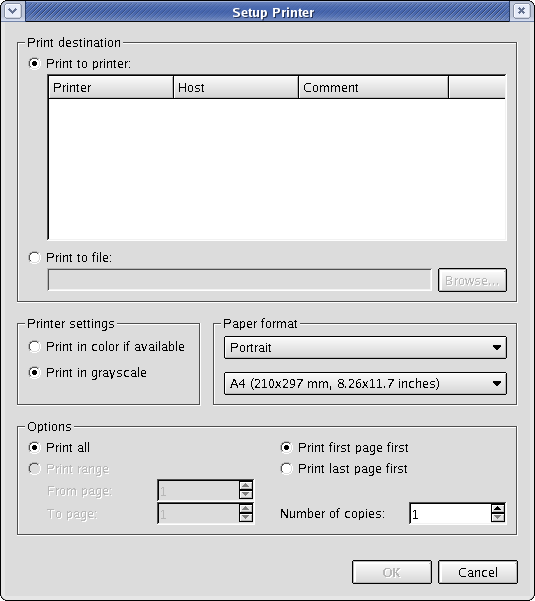
\includegraphics[width=10cm]{Printer}

\caption{Setup Printer}\label{test}

\end{center}

\end{figure}
W"ahlen Sie im Untermenue {\bf Project} den Eintrag {\bf Print} oder in der Symbolleiste den {\bf Drucker}. Im nun aufklappendem Dialog k"onnen Sie Ihre Druckeinstellungen vornehmen und den Druckauftrag an den ausgew"ahlten Drucker mit der Best"atigung durch {\bf OK} schicken.\par
Mit {\bf Cancel} werden die Einstellungen verworfen.\par


%%%%%%%%%%%%%%%%%%%%%%%%%%%%%%%%%%%%%%%%%%%%%%%%%%%%%%%%%%%%%%%%%%%%%%%%%%%%%
\section{Verbindung l"oschen}
W"ahlen Sie die zul"oschende Verbindung mit der rechten Mousetaste aus. Im Kontextmenue w"ahlen Sie nun den Eintrag {\bf Remove} und die Verbindung wird unwiderruflich gel"oscht.
Alternativ k"onnen Sie die zul"oschende Verbindung mit der linken Mousetaste ausw"ahlen und danach das Symbol {\bf l"oschen} in der Symbolleiste oder die {\bf Enfernen} Taste dr"ucken. 


%%%%%%%%%%%%%%%%%%%%%%%%%%%%%%%%%%%%%%%%%%%%%%%%%%%%%%%%%%%%%%%%%%%%%%%%%%%%%
\section{Verbindung routen}
\subsection{Verbindung automatisch routen}
Es gibt zwei verschiedene M"oglichkeiten des automatischen Routens:
\begin{itemize}
\item der Default Router ist der Standartrouter der automatisch beim erzeugen einer Verbindung benutzt wird.
\item der Smart Router kann nach Erzeugung einer Verbindung eingesetzt werden, um eventuell "uberlappende Verbindungen "uberlappungsfrei darzustellen.
\end{itemize}
Wenn Sie eine Verbindung automatisch routen m"ochten, w"ahlen Sie die Verbindung mit rechten Mousetaste aus,w"ahlen Sie im Kontextmenue den Eintrag {\bf Routen} und klicken Sie unter {\bf Routen} auf den gew"unschte Router ({\bf Default Router} oder {\bf Smart Router}).

\subsection{Verbindung manuell routen}
Zum manuellen Routen m"ussen Sie die Verbindung mit der linken Mousetaste ausw"ahlen. Nun k"onnen Sie mit gedr"uckter Mousetaste einen Verbindungsabschnitt entweder horizontal oder vertikal verschieben. Das hei"st ein horizontaler Verbindungsabschnitt kann nur vertikal verschoben werden und ein vertikaler Verbindungsabschnitt nur horizontal. Beim Verschieben der einzelnen Abschnitte werden die anh"angenden Linien automatisch nachgezogen, sodass eine Verbindung immer bestehen bleibt.



%%%%%%%%%%%%%%%%%%%%%%%%%%%%%%%%%%%%%%%%%%%%%%%%%%%%%%%%%%%%%%%%%%%%%%%%%%%%%

\section{Module}

\subsection{Module erzeugen}
Module, wie CPUs, Cores etc. k"onnen Sie per Drag n Drop aus der Modulbibliothek in das Arbeitsfenster gezogen werden und dadurch erzeugt werden. Wenn Sie ein Modul ins Arbeitsfenster gezogen haben und die Mousetaste wieder loslassen, wird automatisch das Konfigurationsfenster f"ur das Modul ge"offnet. Hier haben Sie die M"oglichkeit verschiedene Einstellungen vornehmen (siehe {\bf Konfiguration von Modulen}).


%%%%%%%%%%%%%%%%%%%%%%%%%%%%%%%%%%%%%%%%%%%%%%%%%%%%%%%%%%%%%%%%%%%%%%%%%%%%%
\subsection{Module miteinander verbinden}
Hierzu klicken Sie mit der linken Mousetaste auf den Pin des Moduls und lassen Sie die Mousetaste gedr"uckt. Die Verbindungsm"oglichkeiten werden nun gr"un angezeigt. Sie k"onnen jetzt mit dem Mousezeiger an ein Pin eines anderen Moduls andocken. Dabei muss die linke Mousetaste immer gedr"uckt bleiben. Nachdem Sie am Pin angedockt haben, k"onnen Sie die Mousetaste wieder los lassen und die Verbindung (Connector) wird nun automatisch gezogen. Verbindungen k"onnen nur durch senkrechte oder waagrechte Linien dargestellt werden.


%%%%%%%%%%%%%%%%%%%%%%%%%%%%%%%%%%%%%%%%%%%%%%%%%%%%%%%%%%%%%%%%%%%%%%%%%%%%%
\subsection{Module in Arbeitsfenster verschieben}
W"ahlen Sie das Modul mit der linken Mousetaste aus, lassen Sie Taste gedr"uckt und verschieben das Modul in Arbeitsfenster bis Sie die gew"unschte Position haben. Dabei werden die Verbindungen, die an diesem Modul h"angen automatisch mitgeroutet.


%%%%%%%%%%%%%%%%%%%%%%%%%%%%%%%%%%%%%%%%%%%%%%%%%%%%%%%%%%%%%%%%%%%%%%%%%%%%%
\subsection{Modul kopieren und einf"ugen}
Wenn Sie mehrere identische Module f"ur Ihr Layout ben"otigen eignet sich dazu die "'copy and paste"' Funktion. Hierzu w"ahlen Sie das Modul mit der rechten Mousetaste aus. Im Kontextmenue w"ahlen Sie den Eintrag {\bf Copy}. Wenn Sie nun mit der linken Mousetaste auf ein freies Feld in Arbeitsfenster
klicken, k"onnen Sie im Kontextmenue den Eintrag {\bf Paste} w"ahlen, um eine Kopie des ausgew"ahlten Moduls zu erzeugen.
Die Kopie wird automatisch im linken oberen Rand des Arbeitsfensters positioniert.\par
Altenativ k"onnen Sie diese Aktion auch "uber die Menueleiste bzw. Symbolleiste ausf"uhren. 


%%%%%%%%%%%%%%%%%%%%%%%%%%%%%%%%%%%%%%%%%%%%%%%%%%%%%%%%%%%%%%%%%%%%%%%%%%%%%
\subsection{Modul ausschneiden und einf"ugen}
Hierbei gehen Sie wie zuvor im Abschnitt "'Module kopieren und einf"ugen"' vor, mit der Aunahme, dass Sie statt der Aktion {\bf Copy} die Aktion {\bf Cut} w"ahlen. \par
Wenn ein Modul ausgeschnitten wird, werden alle Verbindungen mit diesem Modul unwiderruflich gel"oscht.


%%%%%%%%%%%%%%%%%%%%%%%%%%%%%%%%%%%%%%%%%%%%%%%%%%%%%%%%%%%%%%%%%%%%%%%%%%%%%
\subsection{Modul l"oschen}
W"ahlen Sie das zul"oschende Modul mit der rechten Mousetaste aus. Im Kontextmenue w"ahlen Sie den Eintrag {\bf Remove} und das Modul wird unwiderruflich gel"oscht.\par
Altenativ k"onnen Sie f"ur das ausgew"ahlte Modul diese Aktion auch "uber die Menueleiste bzw. Symbolleiste ausf"uhren.\par
Wenn ein Modul gel"oscht wird, werden alle Verbindungen mit diesem Modul auch unwiderruflich gel"oscht.


%%%%%%%%%%%%%%%%%%%%%%%%%%%%%%%%%%%%%%%%%%%%%%%%%%%%%%%%%%%%%%%%%%%%%%%%%%%%%
\subsection{Module konfigurieren}
Beim erzeugen eines Moduls wird ein Kofigurationsdialog automatisch ge"offnet. Hier haben Sie je nach Modul verschiedene Konfigurationsm"oglichkeiten. Der Konfigurationsdialog kann auch sp"ater ge"offnet werden. Dazu w"ahlen Sie das zu konfigurierende Modul mit der rechten Mousetaste aus und w"ahlen im Kontextmenue den Eintrag {\bf Configuration} oder ein Doppelklick auf das Modul.\par
Alternativ dazu k"onnen Sie f"ur das ausgew"ahlte Modul die Funktion auch "uber die Menueleiste oder Symbolleiste ausf"uhren. \par
\par
Mit {\bf OK} werden die Einstellungen f"ur das Modul gespeichert und der Dialog wird geschlossen.\par
Mit {\bf Apply} werden die Einstellungen "ubernommen.\par
Mit {\bf Cancel} werden die Einstellungen verworfen und der Dialog wird geschlossen.\par 



\subsection{I/O Block konfigurieren}
\begin{figure}[htbp]

\begin{center}

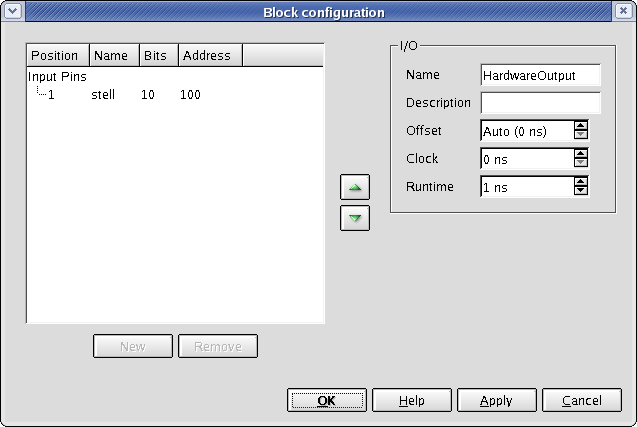
\includegraphics[width=10cm]{OutputBlockConfiguration}

\caption{I/O Block Configuration}\label{test}

\end{center}

\end{figure}
\subsubsection{Modulname "andern}
Im Textfeld {\bf Name} k"onnen Sie den neuen Namen des Moduls eingeben.
\subsubsection{Modul beschreiben}
Im Textfeld {\bf Description} k"onnen Sie Beschreibungen oder Komentare zum Modul eingeben.
\subsubsection{Neue Pins erzeugen}
In der Pinbibliothek k"onnen modulabh"angig drei verschiedene Arten von Pins ("'Episodic Pin"', "'Input Pin"' und "'Output Pin"') verwaltet werden. Je nach Pinart w"ahlen Sie in der Bibliothek die entsprechende Kategorie. Dabei wird der {\bf New} Button aktiviert. Mit einem Kick auf den aktivierten {\bf New} Button wird ein neuer Pin erzeugt. \par
\subsubsection{Pins l"oschen}
W"ahlen Sie in der Pinbibliothek den zu l"oschende Pin aus. Der {\bf Remove} Button wird nun aktiviert. Mit einem Mouseklick auf den {\bf Remove} Button wird der Pin gel"oscht.
\subsubsection{"Anderungen an Pins vornehmen}
W"ahlen Sie in der Pinbibliothek den zu "andernde Pin.\par
Unter der Spalte {\bf Name} k"onnen Sie dem Pin einen Namen geben oder einen vorhandenen Namen "andern.\par
Unter der Spalte {\bf Bits} k"onnen Sie die Anzahl der Bits f"ur ein Pin "andern.\par
Unter der Spalte {\bf Address} k"onnen Sie eine Adressierung f"ur die Input-Pins und Output-Pins vornehmen.\par
\subsubsection{Offset eingeben}
Um das Offset einzugeben, k"onnen Sie entweder direkt mit der Mouse ins Textfeld {\bf Offset} klicken und die Offsetzeit in Nanosekunden eingeben oder Sie benutzen die Pfeiltasten neben dem Textfeld. 
\subsubsection{Takt eingeben}
Um den Takt einzugeben, k"onnen Sie entweder direkt mit der Mouse ins Textfeld {\bf Clock} klicken und die Taktfrequenz in Nanosekunden eingeben oder Sie benutzen die Pfeiltasten neben dem Textfeld. 
\subsubsection{Laufzeit eingeben}
Um die Laufzeit einzugeben, k"onnen Sie entweder direkt mit der Mouse ins Textfeld{\bf Runtime} klicken und die Laufzeit in Nanosekunden eingeben oder Sie benutzen die Pfeiltasten neben dem Textfeld. 




\subsection{CPU konfigurieren}
\begin{figure}[htbp]

\begin{center}

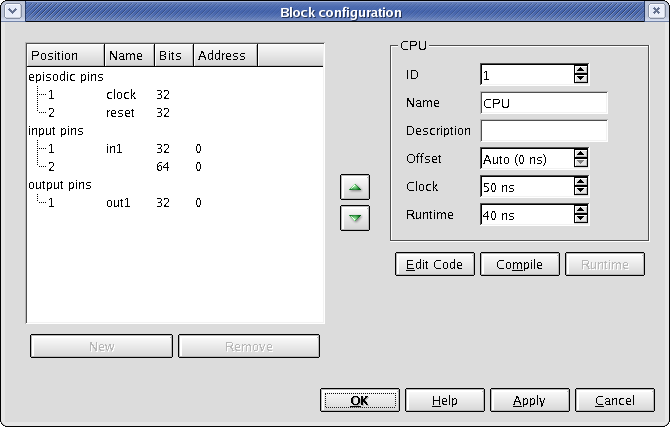
\includegraphics[width=10cm]{CPUConfiguration}

\caption{CPU Configuration}\label{test}

\end{center}

\end{figure}
\subsubsection{Neue Pins erzeugen}
In der Pinbibliothek werden drei verschiedene Arten von Pins ("'Episodic Pin"', "'Input Pin"' und "'Output Pin"') verwaltet. Je nach Pinart w"ahlen Sie in der Bibliothek die entsprechende Kategorie. Dabei wird der {\bf New} Button aktiviert. Mit einem Kick auf den aktivierten {\bf New} Button wird ein neuer Pin erzeugt. \par
\subsubsection{Pins l"oschen}
W"ahlen Sie in der Pinbibliothek den zu l"oschende Pin aus. Der {\bf Remove} Button wird nun aktiviert. Mit einem Mouseklick auf den {\bf Remove} Button wird der Pin gel"oscht.
\subsubsection{"Anderungen an Pins vornehmen}
W"ahlen Sie in der Pinbibliothek den zu "andernde Pin.\par
Unter der Spalte {\bf Name} k"onnen Sie dem Pin einen Namen geben oder einen vorhandenen Namen "andern.\par
Unter der Spalte {\bf Bits} k"onnen Sie die Anzahl der Bits f"ur ein Pin "andern.\par
Unter der Spalte {\bf Address} k"onnen Sie eine Adressierung f"ur die CPU-Pins vornehmen.\par
\subsubsection{ID eingeben}
Jeder CPU kann eine ID (d.h. eine Nummer von 0 - 99) vergeben werden, dazu k"onnen Sie entweder direkt mit der Mouse ins Textfeld {\bf ID} klicken und die Nummer eingeben oder Sie benutzen die Pfeiltasten neben dem Textfeld.
\subsubsection{CPU-Name "andern}
Im Textfeld {\bf Name} k"onnen Sie den neuen Namen der CPU eingeben.
\subsubsection{CPU beschreiben}
Im Textfeld {\bf Description} k"onnen Sie Beschreibungen oder Komentare zur CPU eingeben.
\subsubsection{Offset eingeben}
Um das Offset einzugeben, k"onnen Sie entweder direkt mit der Mouse ins Textfeld {\bf Offset} klicken und die Offsetzeit in Nanosekunden eingeben oder Sie benutzen die Pfeiltasten neben dem Textfeld. 
\subsubsection{Takt eingeben}
Um den Takt einzugeben, k"onnen Sie entweder direkt mit der Mouse ins Textfeld {\bf Clock} klicken und die Taktfrequenz in Nanosekunden eingeben oder Sie benutzen die Pfeiltasten neben dem Textfeld. 
\subsubsection{Laufzeit eingeben}
Um die Laufzeit einzugeben, k"onnen Sie entweder direkt mit der Mouse ins Textfeld{\bf Runtime} klicken und die Laufzeit in Nanosekunden eingeben oder Sie benutzen die Pfeiltasten neben dem Textfeld. 
\subsubsection{Die CPU-Programmcode schreiben}
Zum Schreiben von CPU-Programmcode wird ein externer Editor aufgerufen, wenn Sie im Konfigurationsdialog den Button {\bf Edit Code} dr"ucken. Im Editor k"onnen Sie dann den Qellcode f"ur die CPU niederschreiben und abspeichern.
 



\subsection{Core konfigurieren}
\begin{figure}[htbp]

\begin{center}

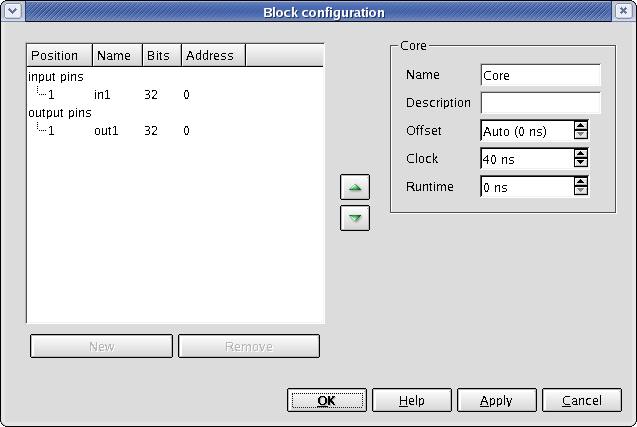
\includegraphics[width=10cm]{CoreBlockConfiguration}

\caption{Core Configuration}\label{test}

\end{center}

\end{figure}
\subsubsection{Neue Pins erzeugen}
In der Pinbibliothek werden drei verschiedene Arten von Pins ("'Episodic Pin"', "'Input Pin"' und "'Output Pin"') verwaltet. Je nach Pinart w"ahlen Sie in der Bibliothek die entsprechende Kategorie. Dabei wird der {\bf New} Button aktiviert. Mit einem Kick auf den aktivierten {\bf New} Button wird ein neuer Pin erzeugt. \par
\subsubsection{Pins l"oschen}
W"ahlen Sie in der Pinbibliothek den zu l"oschende Pin aus. Der {\bf Remove} Button wird nun aktiviert. Mit einem Mouseklick auf den {\bf Remove} Button wird der Pin gel"oscht.
\subsubsection{"Anderungen an Pins vornehmen}
W"ahlen Sie in der Pinbibliothek den zu "andernde Pin.\par
Unter der Spalte {\bf Name} k"onnen Sie dem Pin einen Namen geben oder einen vorhandenen Namen "andern.\par
Unter der Spalte {\bf Bits} k"onnen Sie die Anzahl der Bits f"ur ein Pin "andern.\par
Unter der Spalte {\bf Address} k"onnen Sie eine Adressierung f"ur Coreblock-Pins vornehmen.\par
\subsubsection{Coreblockname "andern}
Im Textfeld {\bf Name} k"onnen Sie den neuen Namen des Coreblocks eingeben.
\subsubsection{Coreblock beschreiben}
Im Textfeld {\bf Description} k"onnen Sie Beschreibungen oder Komentare zum Coreblock eingeben.
\subsubsection{Offset eingeben}
Um das Offset einzugeben, k"onnen Sie entweder direkt mit der Mouse ins Textfeld {\bf Offset} klicken und die Offsetzeit in Nanosekunden eingeben oder Sie benutzen die Pfeiltasten neben dem Textfeld. 
\subsubsection{Takt eingeben}
Um den Takt einzugeben, k"onnen Sie entweder direkt mit der Mouse ins Textfeld {\bf Clock} klicken und die Taktfrequenz in Nanosekunden eingeben oder Sie benutzen die Pfeiltasten neben dem Textfeld. 
\subsubsection{Laufzeit eingeben}
Um die Laufzeit einzugeben, k"onnen Sie entweder direkt mit der Mouse ins Textfeld{\bf Runtime} klicken und die Laufzeit in Nanosekunden eingeben oder Sie benutzen die Pfeiltasten neben dem Textfeld. 




\subsection{Mux konfigurieren}
\begin{figure}[htbp]

\begin{center}

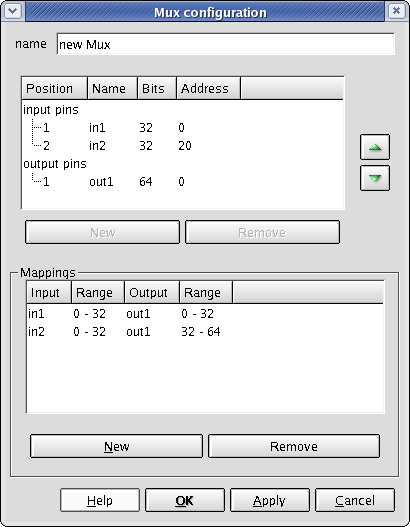
\includegraphics[width=10cm]{MuxConfiguration}

\caption{Mux Configuration}\label{test}

\end{center}

\end{figure}
\subsubsection{Muxname "andern}
Im Textfeld {\bf Name} k"onnen Sie den neuen Namen des Mux eingeben.
\subsubsection{Neue Pins erzeugen}
In der Pinbibliothek werden drei verschiedene Arten von Pins ("'Episodic Pin"', "'Input Pin"' und "'Output Pin"') verwaltet. Je nach Pinart w"ahlen Sie in der Bibliothek die entsprechende Kategorie. Dabei wird der {\bf New} Button aktiviert. Mit einem Kick auf den aktivierten {\bf New} Button wird ein neuer Pin erzeugt. \par
\subsubsection{Pins l"oschen}
W"ahlen Sie in der Pinbibliothek den zu l"oschende Pin aus. Der {\bf Remove} Button wird nun aktiviert. Mit einem Mouseklick auf den {\bf Remove} Button wird der Pin gel"oscht.
\subsubsection{"Anderungen an Pins vornehmen}
W"ahlen Sie in der Pinbibliothek den zu "andernde Pin.\par
Unter der Spalte {\bf Name} k"onnen Sie dem Pin einen Namen geben oder einen vorhandenen Namen "andern.\par
Unter der Spalte {\bf Bits} k"onnen Sie die Anzahl der Bits f"ur ein Pin "andern.\par
Unter der Spalte {\bf Address} k"onnen Sie eine Adressierung Mux-Pins vornehmen.\par



\end{document}
